\section{Certificate Genertion System}

Apart from the major project i.e OSM I have done another project "Certificate Generation System".

Certificate Generation System is a portable application used to Generate Certificate for single candidate providing his/her details along with image,
As well as for Batch/Number of candidates by simply providing the CSV format file (containing details of every candidate) along with candidate images.

CSV(Character Separated File) is a simple file format used to store tabular data, such as a spreadsheet or database. Files in the CSV format can be imported to and exported from programs that store data in tables, such as Microsoft Excel or OpenOffice Calc.

INSTALLATION/SETUP

This application is a portable application used to Generate Certificate for single candidate providing his/her details along with image,
As well as for Batch/Number of candidates by simply providing the CSV format file (containing details of every candidate) along with candidate images in a compressed (tar.gz or zip) folder.
Requirements(automatically installed during setup)

    Apache web server
    php interpreter
    unoconv
    python3-uno

USER MANUAL

As the Name "Certificate Generation System" Implies this application is used to generate certificate in an automated manner in few steps:

    Select Design from the images shown on the first page. ( Put mouse pointer over the image to see larger view. )

\begin{figure}[!ht]
\centering
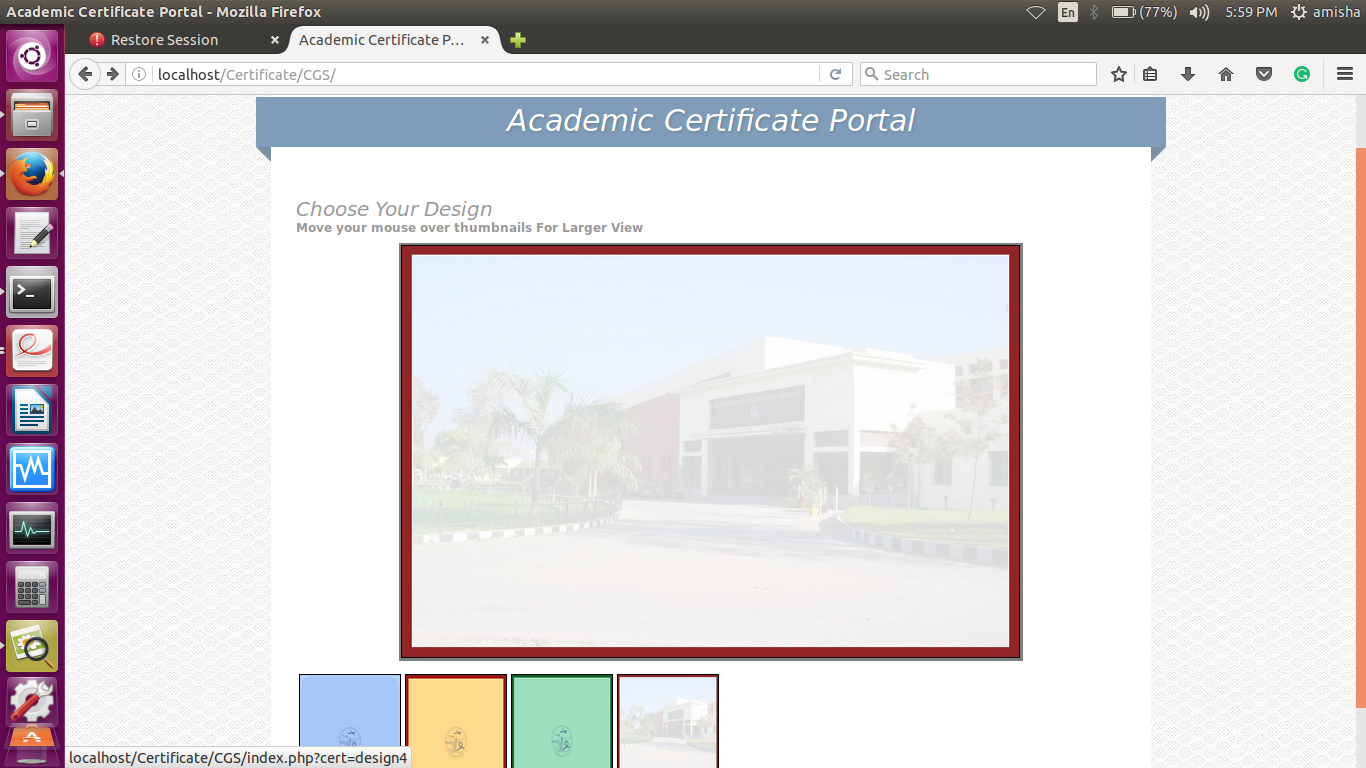
\includegraphics[width=0.7\textwidth]{input/images/cgs/cgs1.png}
\caption{Academic Portal}
\hspace{-1.5em}
\end{figure}


    Next Page will be page for entering Institute Details.


    Fill in the details of institution for which the certificate(s) is to be made.

    Place mouse pointer over Input box te see an example for that input.
\begin{figure}[!ht]
\centering
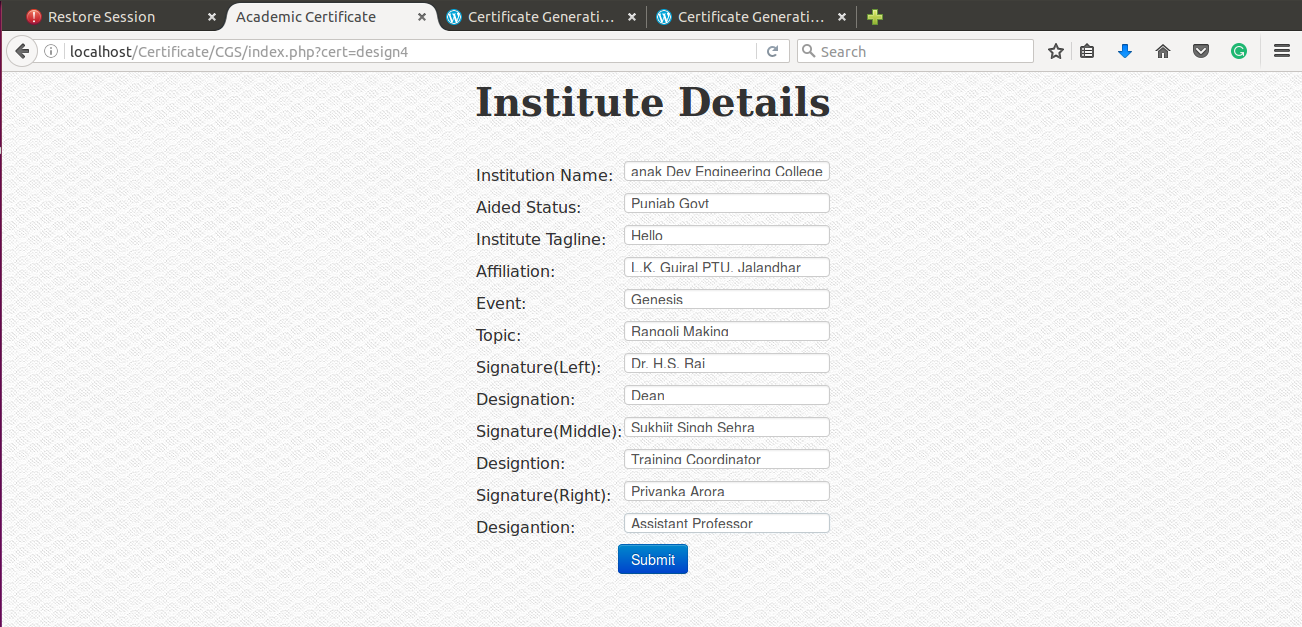
\includegraphics[width=0.7\textwidth]{input/images/cgs/cgs2.png}                  
\caption{Institute Details}
\hspace{-1.5em}
\end{figure}


    Next page will show two options

    Manual Entry -> Select it for Generating Certificate for Single candidate.

    Upload Csv File -> Select it for Generating certificate for more than 1 candidate by providing their details in Csv file.
    Manual Entry
\begin{figure}[!ht]
\centering
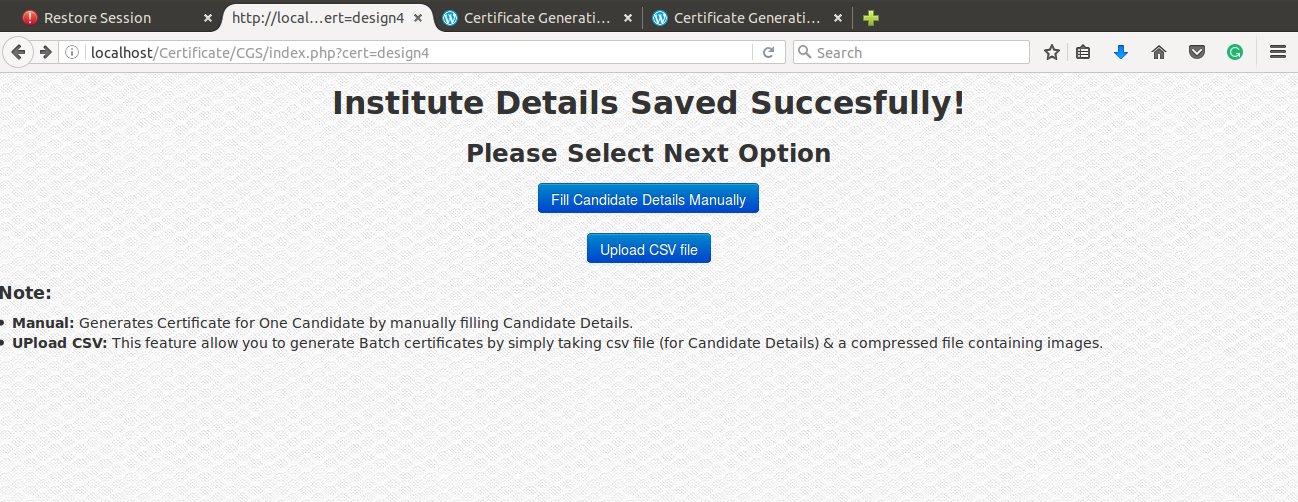
\includegraphics[width=0.7\textwidth]{input/images/cgs/cgs3.png}                  
\caption{Select Manual Option}
\hspace{-1.5em}
\end{figure}

    On Selecting Manual Entry Next page will open containing input boxes for candidate Details.

    Enter the details and select the image also.

    Live Image Selector

    Next you will be displayed your selected image and a selection box.

\begin{figure}[!ht]
\centering
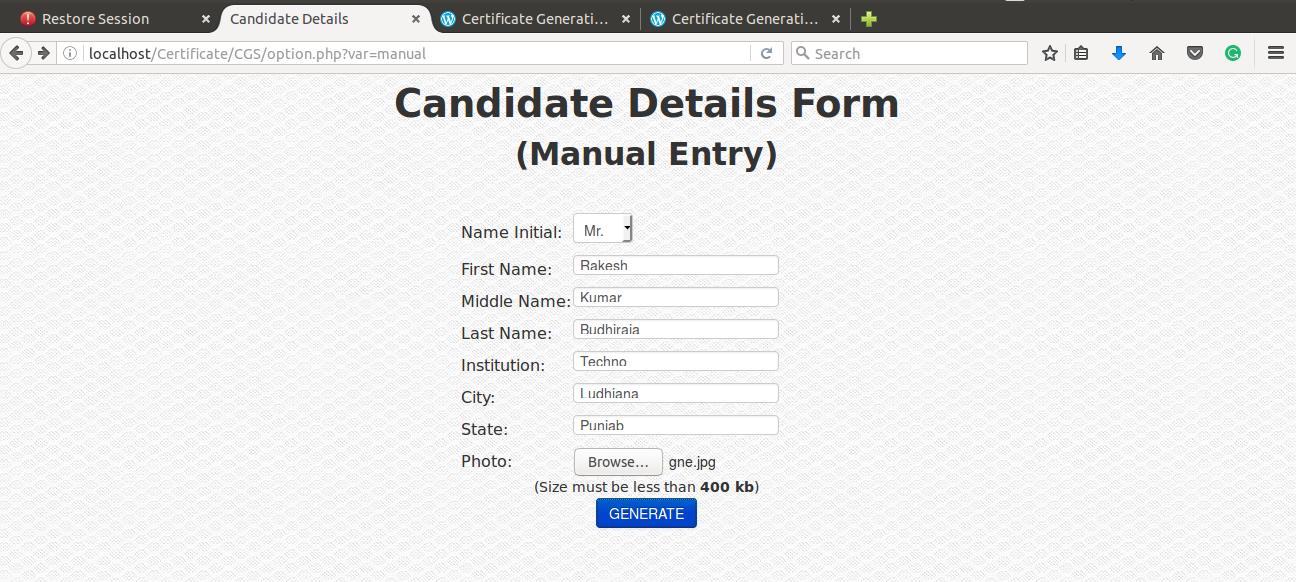
\includegraphics[width=0.7\textwidth]{input/images/cgs/cgs4.png}                  
\caption{Candidate Details Form}
\hspace{-1.5em}
\end{figure}

    Resize and move the selection box to desired position and size.

\begin{figure}[!ht]
\centering
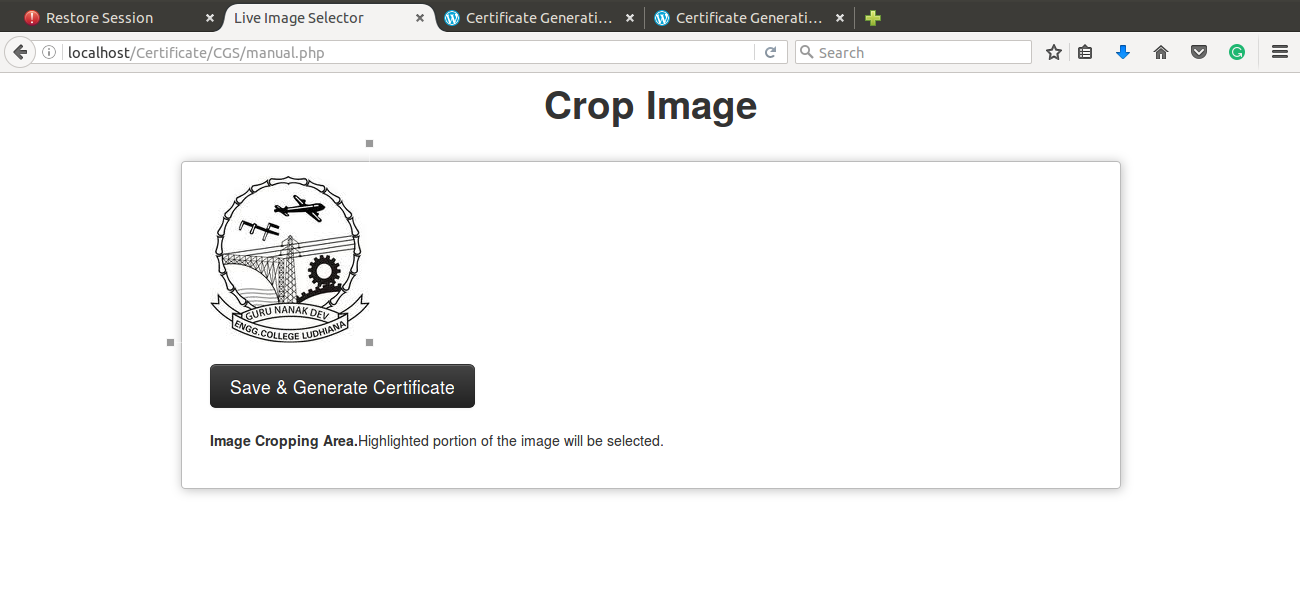
\includegraphics[width=0.7\textwidth]{input/images/cgs/cgs5.png}                  
\caption{Crop Image}
\hspace{-1.5em}
\end{figure}

    Download

    Thats it your certificate is generated and can be downloaded in two formats

    -> odt ('O'penOffice 'D'ocument 'T'ext)

    -> pdf ('P'ortable 'D'ocument 'F'ormat)

\begin{figure}[!ht]
\centering
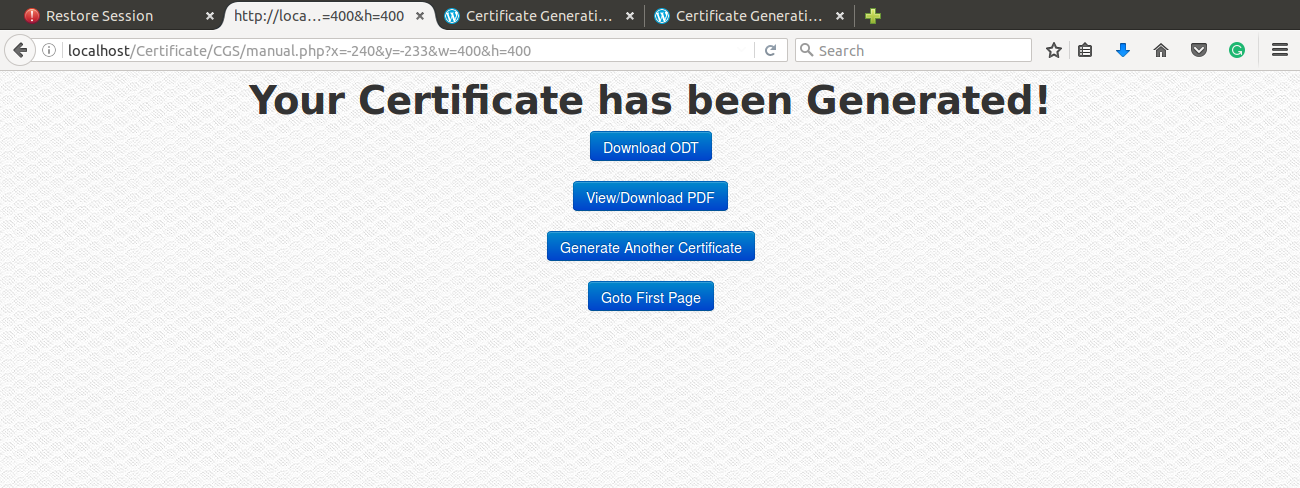
\includegraphics[width=0.7\textwidth]{input/images/cgs/cgs6.png}                  
\caption{Download Certificate}
\hspace{-1.5em}
\end{figure}

\begin{figure}[!ht]
\centering
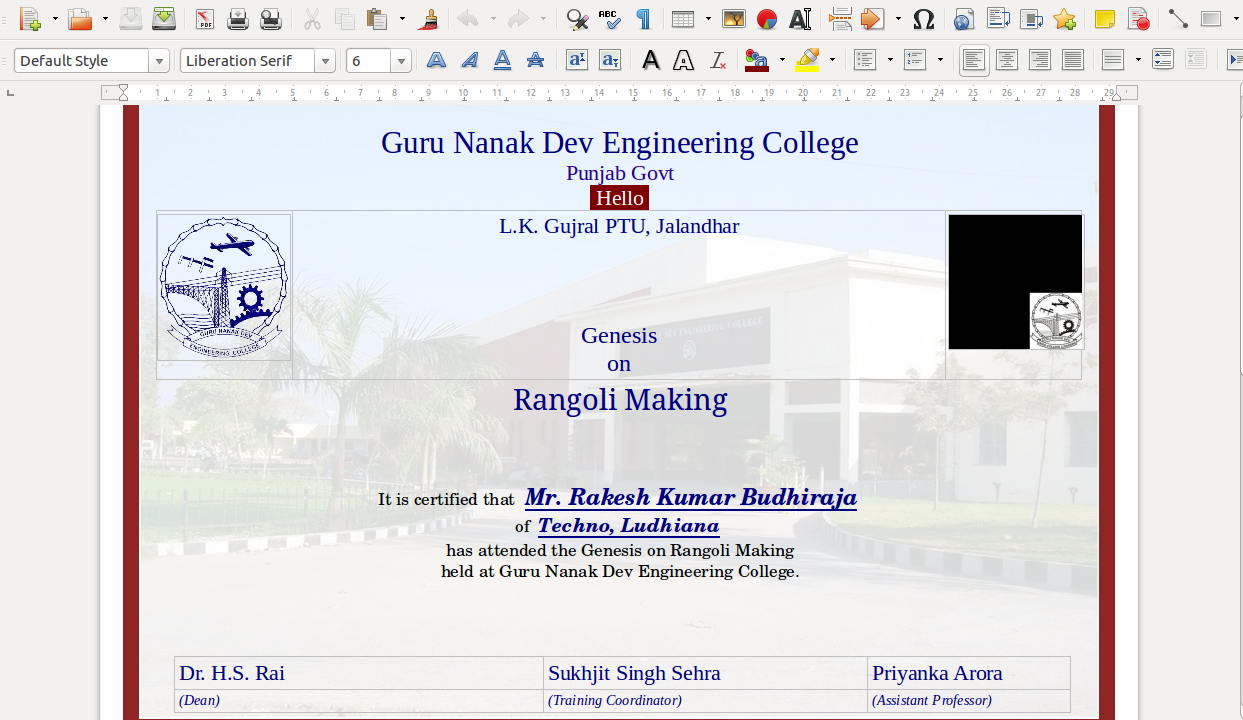
\includegraphics[width=0.7\textwidth]{input/images/cgs/cgs8.png}                 
\caption{Certificate odt file}
\hspace{-1.5em}
\end{figure}


    Also by clicking on "Generate Another Ceritificate" you can generate another certificate

    with same design & institute details and different Candidate Details.

    And by clicking on "Goto First Page" you can again start from Design Selection Page.
    Upload csv file

    On selecting 'Upload csv File' Next page will open containing the conditions for the files

    to be uploaded for certificate generation.
\begin{figure}[!ht]
\centering
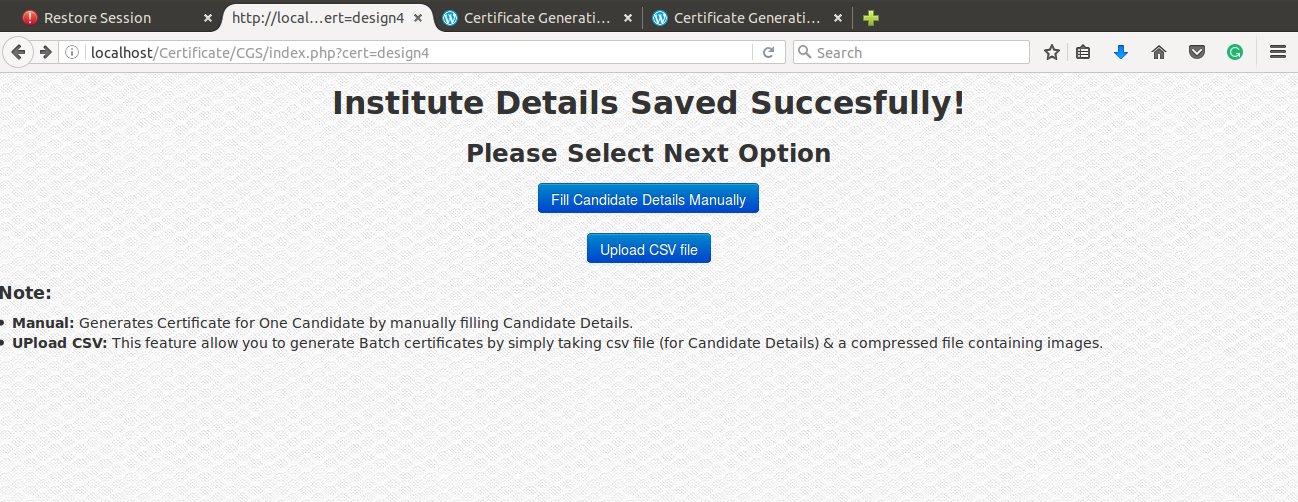
\includegraphics[width=0.7\textwidth]{input/images/cgs/cgs3.png}                  
\caption{Choose csv Option}
\hspace{-1.5em}
\end{figure}
    A sample file can be downloaded from the link provided in the 'Note' in the instructions on page.

    Sample file is a zip file named sample.zip containing the csv file and tar.gz file for images.

    Extract it and then sample certificates can be produced using 'sample.csv' and 'images.tar.gz' files.

\begin{figure}[!ht]
\centering
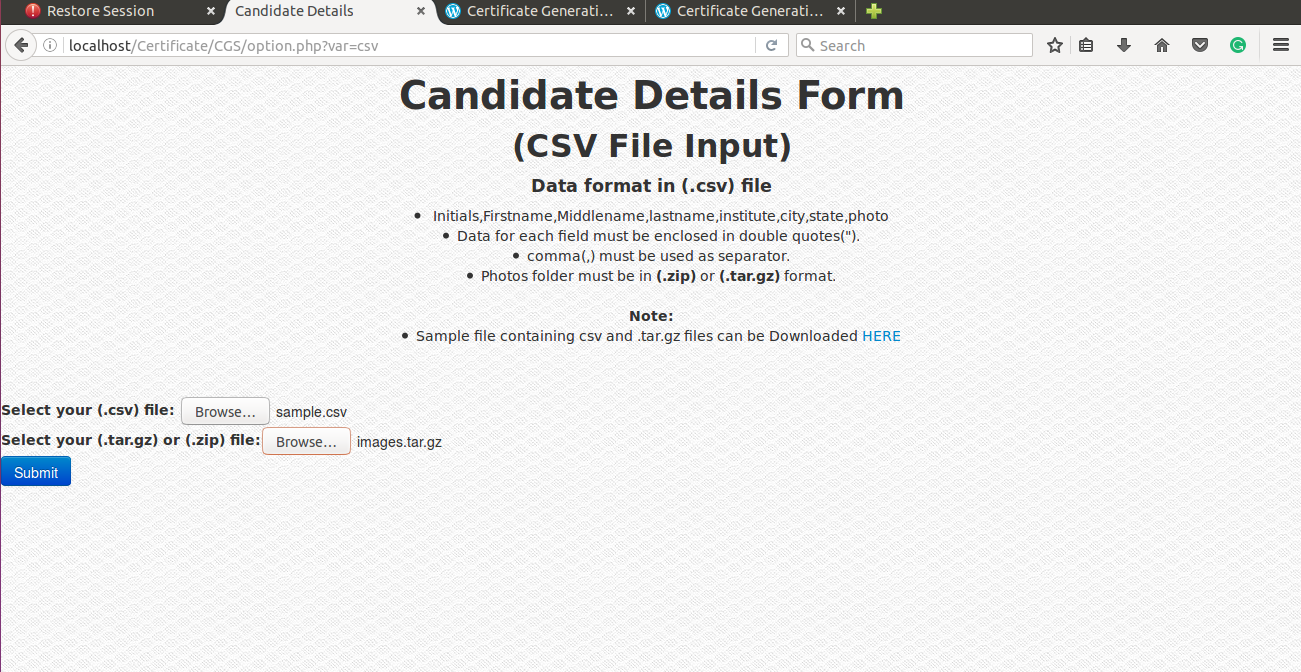
\includegraphics[width=0.7\textwidth]{input/images/cgs/cgs9.png}                 
\caption{Candidate Details Form}
\hspace{-1.5em}
\end{figure}


    That's it your certificate file is produced for all the candidates provided in the csv data file.

Produced Certificate file can be downloaded in two formats again.

-> odt ('O'penOffice 'D'ocument 'T'ext)

-> pdf ('P'ortable 'D'ocument 'F'ormat)
\begin{figure}[!ht]
\centering
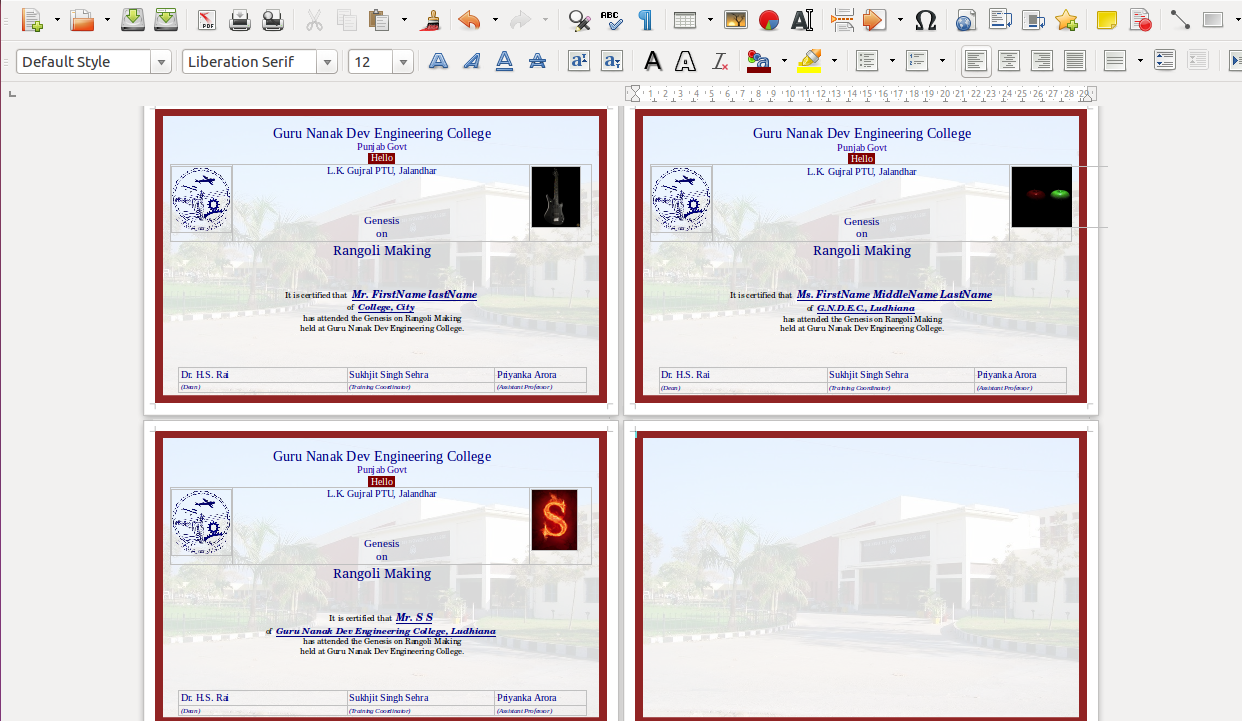
\includegraphics[width=0.7\textwidth]{input/images/cgs/cgs14.png}                  
\caption{Odt file through csv}
\hspace{-1.5em}
\end{figure}
